
\chapter{Symplectic算法在GPU上的实现}
\label{chap:symplectic}

数值模拟在束流动力学研究和加速器设计中非常重要。目前,主流的模拟软件都是用质点网格法(PIC)求解空间电荷效应\cite{PIC_Birdsall1991, PIC_friedman1992, PIC_ji2000, PIC_ji2004, PIC_Amundson2006229, PIC_tracewin2014, PIC_beampath2005}。
PIC算法是求解空间电荷效应非常快速有效的方法,在PIC算法中,粒子首先被根据位置权重到网格上,然后根据网格上的电荷密度求解泊松方程,得到网格上的电势,从而得到网格上的电场,再根据粒子位置反推出粒子所处位置的电场。使用这种方法,计算复杂度由直接的粒子-粒子方法的 $N_p^2$ 降低到了$\alpha N_p + \beta N_{cells}\log{N_{cells}}$。其中 $N_p$ 是粒子数,而$N_{cells}$ 是网格点数目。

然而,PIC算法需要将粒子权重到网格上,不可避免的会带来网格热噪声,因此PIC算法是否可以保障辛条件在目前仍然有较大的争议。如果不能报障辛条件,那么计算就会被引入一些数值算法带来的非物理的效应。这些效应对最终的强流束流物理的分析和讨论会带来一些干扰。因此,在需要长程模拟(比如环形加速器)的物理分析中,我们需要一种保辛的算法。

最初,保辛算法本身是为了保障哈密顿系统中的辛条件而被研究 \cite{symplectic_channel1990, symplectic_yoshida1990}。后来,无网格保辛多粒子追踪模型被引入到加速器研究和模拟中,作为在长距离模拟中空间电荷求解器 \cite{symplectic_ji2017}。
这种模型并不利用网格,而是利用高阶分解来求解空间电荷效应。
相比PIC算法,这种方法能够显著的降低由于网格数值噪声带来的发射度增长。
然而,虽然能够保证辛条件,这种算法也有缺陷,最显著的就是计算量要大得多。
无网格算法的计算复杂度为 $\alpha N_p * N_{modes}$ ,其中$N_{modes}$为分解的阶数,在通常模拟中我们一般使用$16 \times 16 \times 16$ 阶,在这种配置下花费的时间比PIC算法要高两到三个数量级。
所以我们必须提高这个算法的运行速度,以提高算法的实用性。

幸运的是,无网格算法很适合并行,有很好的可扩展性。这种特性非常适合使用GPU进行加速计算。通过使用CUDA和GPU,可以显著加快无网格粒子跟踪代码的运行速度。当运行在单个GTX 1060时,与CPU串行相比,GPU代码实现了超过400倍的加速。此外,加速比会随着GPU的数目线性增长。

在接下来的这一章中, 我们将会首先在小节\ref{section:theory} 中介绍保辛空间电荷算法。接下来我们会在小节\ref{section:code}中介绍算法在GPU上的代码结构和优化。在小节 \ref{section:performance}中,我们会讨论代码的加速比. 在小节\ref{section:simulation}中,我们展示了使用这个代码的一个应用实例。

\section{Symplectic算法}\label{section:theory}

在束流动力学模拟中,当且仅当雅可比矩阵$M_i$满足以下条件时,传输矩阵$ m_i $才是保辛的\cite{accelerator2004lee, accelerator2013chao}:
\begin{equation}
M_{i}^{T}J{{M}_{i}}=J
\end{equation}
其中,$J$ 是如下 $6N\times6N$ 的矩阵:
\begin{equation}
J=\left(
  \begin{array}{cc}
     0 & I \\
    -I & 0 \\
  \end{array}
\right)
\end{equation}

对于考虑其空间电荷力的多粒子系统,哈密尔顿量可以写为:
\begin{equation}
H={{H}_{1}}+{{H}_{2}}
\end{equation}
其中
\begin{eqnarray}
% \nonumber to remove numbering (before each equation)
  {H}_{1} &=& \sum\limits_{i}{{p_{i}^{2}}/{2}\;}+\sum\limits_{i}{q\psi ({{r}_{i}})} \\
  {H}_{2} &=& \frac{1}{2}\sum\limits_{i}{\sum\limits_{j}{q\varphi ({{r}_{i}},{{r}_{j}})}}
\end{eqnarray}

其中${{H}_{1}}$ 只包含外场信息,而 ${{H}_{2}}$ 只包括空间电荷效应。根据${{H}_{1}}$ 和 ${{H}_{2}}$ 得到的两个传输矩阵 ${{m}_{1}}$和 ${{m}_{2}}$,一个二阶传输矩阵$m\left( \tau  \right)$可以被定义为:
\begin{equation}
m\left( \tau  \right)={{m}_{1}}\left( \tau /2 \right){{m}_{2}}\left( \tau  \right){{m}_{1}}\left( \tau /2 \right)
\end{equation}

如果$ {{m} _ {1}} $和$ {{m} _ {2}} $都是保辛的,那么$ m $就是保辛的。在大多数加速器元件中,我们可以通过单粒子动力学获得相应的外场传输矩阵$ {{m} _ {1}} $,而内场传输矩阵$ {{m} _ {2}} $可以写为:
\begin{eqnarray}
 {{r}_{i}}(\tau ) &=& {{r}_{i}}(0) \\
 {{p}_{i}}(\tau ) &=& {{p}_{i}}(0)-\frac{\partial {{H}_{2}}(r)}{\partial {{r}_{i}}}\tau
\end{eqnarray}
其雅克比矩阵为:
\begin{equation}
{{M}_{2}}=\left(
\begin{array}{cc}
   I & 0  \\
   L & I  \\
\end{array} \right)
\end{equation}
其中
${{L}_{ij}}=\frac{\partial {{p}_{i}}(\tau )}{\partial {{r}_{j}}}=-\frac{{{\partial }^{2}}{{H}_{2}}(r)}{\partial {{r}_{i}}\partial {{r}_{j}}}\tau$
是一个对称矩阵,所以${{M}_{2}}$满足保辛条件.

对于一个3D束团, ${{H}_{2}}$可以表示为:
\begin{equation}
{{H}_{2}}=\kappa {{\gamma }_{0}}\sum\limits_{i}{\sum\limits_{j}{\varphi ({{r}_{i}},{{r}_{j}})}}
\end{equation}
其中 $\kappa =q/(lm{{C}^{2}}\gamma _{0}^{2}{{\beta }_{0}}),l=C/\omega $。而在束流坐标系下的静电势可以有泊松方程得到:
\begin{equation}
\frac{{{\partial }^{2}}\phi }{\partial {{x}^{2}}}+\frac{{{\partial }^{2}}\phi }{\partial {{y}^{2}}}+\frac{{{\partial }^{2}}\phi }{\partial {{z}^{2}}}=-\frac{\rho }{{{\varepsilon }_{0}}}
\end{equation}
其中边界条件为:
\begin{equation}
\begin{array}{cc}
   \phi (x=0,y,z)=0, & \phi (x=a,y,z)=0  \\
   \phi (x,y=0,z)=0, & \phi (x,y=b,z)=0  \\
   \phi (x,y,z=0)=0, & \phi (x,y,z=c)=0  \\
\end{array}
\end{equation}
其中,$a$,$b$,$c$分别是X,Y,Z方向上的零电势边界长度。如果我们将$c$设的足够大,电势将在无穷远处为零。

泊松方程中的电势$\phi$和电荷密度$\rho$可以展开为:
\begin{eqnarray}
 \rho(x,y,z)&=&\sum\limits_{l=1}^{{{N}_{l}}}{\sum\limits_{m=1}^{{{N}_{m}}}{\sum\limits_{n=1}^{{{N}_{n}}}{{{\rho }^{lmn}}\sin ({{\alpha }_{l}}x)\sin ({{\beta }_{m}}y)\sin ({{\gamma }_{n}}z)}}} \\
 \phi(x,y,z)&=&\sum\limits_{l=1}^{{{N}_{l}}}{\sum\limits_{m=1}^{{{N}_{m}}}{\sum\limits_{n=1}^{{{N}_{n}}}{{{\phi }^{lmn}}\sin ({{\alpha }_{l}}x)\sin ({{\beta }_{m}}y)\sin ({{\gamma }_{n}}z)}}}
\end{eqnarray}
其中 ${N}_{l}$,${N}_{m}$,${N}_{n}$分别为电势和电荷密度在X,Y,Z三个方向上展开的阶数,而 ${\rho }^{lmn}$和 ${\phi }^{lmn}$可以表达为:
\begin{eqnarray}
  {{\rho }^{lmn}}&=&\frac{8}{abc}\int\limits_{0}^{a}{\int\limits_{0}^{b}{\int\limits_{0}^{b}{\rho (x,y,z)\sin ({{\alpha }_{l}}x)\sin ({{\beta }_{m}}y)\sin ({{\gamma }_{n}}z)dxdydz}}} \\
 {{\phi }^{lmn}}&=&\frac{8}{abc}\int\limits_{0}^{a}{\int\limits_{0}^{b}{\int\limits_{0}^{b}{\phi (x,y,z)\sin ({{\alpha }_{l}}x)\sin ({{\beta }_{m}}y)\sin ({{\gamma }_{n}}z)dxdydz}}}
\end{eqnarray}
其中
\begin{equation}
{{\alpha }_{l}}=\frac{l\pi }{a},{{\beta }_{m}}=\frac{m\pi }{b},{{\gamma }_{n}}=\frac{n\pi }{c}
\end{equation}

将上面的展开代入泊松方程,我们可以得到:
\begin{equation}
{{\phi }^{lmn}}=\frac{{{\rho }^{lmn}}}{{{\varepsilon }_{0}}(\alpha _{l}^{2}+\beta _{m}^{2}+\gamma _{n}^{2})}
\end{equation}

据此,我们得到了粒子密度$ \ rho $和电势$ \ phi $之间的关系:
\begin{multline}
\phi (x,y,z)=\frac{1}{{{\varepsilon }_{0}}}\frac{8}{abc}\omega \times \\ \sum\limits_{j=1}^{{{N}_{j}}}{\sum\limits_{l=1}^{{{N}_{l}}}{\sum\limits_{m=1}^{{{N}_{m}}}{\sum\limits_{n=1}^{{{N}_{n}}}{\frac{\sin ({{\alpha }_{l}}{{x}_{j}})\sin ({{\beta }_{m}}{{y}_{j}})\sin ({{\gamma }_{n}}{{z}_{j}})\sin ({{\alpha }_{l}}x)\sin ({{\beta }_{m}}y)\sin ({{\gamma }_{n}}z)}{(\alpha _{l}^{2}+\beta _{m}^{2}+\gamma _{n}^{2})}}}}}
\end{multline}
其中 $\omega $ 是粒子的电荷。

于是哈密顿量 ${{H}_{2}}$可以表示为:
\begin{multline}
{{H}_{2}}=\frac{1}{{{\varepsilon }_{0}}}\frac{8}{abc}\omega \kappa {{\gamma}_{0}} \times \\
\sum\limits_{i=1}^{{{N}_{i}}}{\sum\limits_{j=1}^{{{N}_{j}}}{\sum\limits_{l=1}^{{{N}_{l}}}{\sum\limits_{m=1}^{{{N}_{m}}}{\sum\limits_{n=1}^{{{N}_{n}}}
{\frac{\sin ({{\alpha }_{l}}{{x}_{j}})\sin ({{\beta }_{m}}{{y}_{j}})\sin ({{\gamma }_{n}}{{z}_{j}})\sin ({{\alpha }_{l}}{{x}_{i}})\sin ({{\beta }_{m}}{{y}_{i}})\sin ({{\gamma }_{n}}{{z}_{i}})}{(\alpha _{l}^{2}+\beta _{m}^{2}+\gamma _{n}^{2})}}
}}}}
\end{multline}

我们得到了保辛的空间电荷传输矩阵 ${{m}_{2}}$。 以X方向为例:
\begin{align}
&{{x}_{i}}(\tau )= {{x}_{i}}(0) \\
 \nonumber &{{p}_{xi}}(\tau )= {{p}_{xi}}(0)-\tau \frac{1}{{{\varepsilon }_{0}}}\frac{8}{abc}\omega \kappa {{\gamma }_{0}} \times \\
 &\sum\limits_{j=1}^{{{N}_{j}}}{\sum\limits_{l=1}^{{{N}_{l}}}{\sum\limits_{m=1}^{{{N}_{m}}}{\sum\limits_{n=1}^{{{N}_{n}}}{\frac{{{\alpha }_{l}}\sin ({{\alpha }_{l}}{{x}_{j}})\sin ({{\beta }_{m}}{{y}_{j}})\sin ({{\gamma }_{n}}{{z}_{j}})\cos ({{\alpha }_{l}}{{x}_{i}})\sin ({{\beta }_{m}}{{y}_{i}})\sin ({{\gamma }_{n}}{{z}_{i}})}{(\alpha _{l}^{2}+\beta _{m}^{2}+\gamma _{n}^{2})}}}}}\label{eq:map1}
\end{align}
在Y和Z方向的传输矩阵与之类似。
%\begin{equation}\label{xx}
%\begin{split}
%{{p}_{xi}}(\tau )&={{p}_{xi}}(0)-\frac{\partial {{H}_{2}}(r)}{\partial {{x}_{i}}}\tau  \\
% & ={{p}_{xi}}(0)-\tau \frac{1}{{{\varepsilon }_{0}}}\frac{8}{abc}\omega \kappa {{\gamma }_{0}}\sum\limits_{j=1}^{{{N}_{j}}}{\sum\limits_{l=1}^{{{N}_{l}}}{\sum\limits_{m=1}^{{{N}_{m}}}{\sum\limits_{n=1}^{{{N}_{n}}}{\frac{{{\alpha }_{l}}\sin ({{\alpha }_{l}}{{x}_{j}})\sin ({{\beta }_{m}}{{y}_{j}})\sin ({{\gamma }_{n}}{{z}_{j}})\cos ({{\alpha }_{l}}{{x}_{i}})\sin ({{\beta }_{m}}{{y}_{i}})\sin ({{\gamma }_{n}}{{z}_{i}})}{(\alpha _{l}^{2}+\beta _{m}^{2}+\gamma _{n}^{2})}}}}}
%\end{split}
%\end{equation}

\section{GPU程序结构}            \label{section:code}
在大多数加速元件中,粒子会被推动若干步。在每一步中,粒子将首先被外场传输矩阵传输推动半个时间步长,然后由空间电荷推动一个时间步长,并再次被外场传输矩阵传输推动半个时间步长。
其中,求解空间电荷将消耗整个计算时间的90%以上。 计算空间电荷效应的程序由下面的三个子程序组成,而每个子程序由一个或两个内核组成。
\begin{enumerate}
  \item 遍历三角函数
  \item 计算$\Phi^{lmn}$
  \item 计算$ep_i$并推动粒子
\end{enumerate}

我们对程序进行了许多优化,使其更适合GPU架构,程序的性能得到显着改善。 每个子程序的优化策略各不相同,下面介绍各个内核的详细优化策略。
\subsection{遍历三角函数}
根据粒子的位置,我们首先计算每个粒子的三角函数临时变量。设:
\begin{equation}
\begin{array}{cc}
    S^{l}_j =sin(\alpha_l x_j), & C^{l}_j =cos(\alpha_l x_j)  \\
    S^{m}_j =sin(\alpha_m x_j), & C^{m}_j =cos(\alpha_m x_j)  \\
    S^{n}_j =sin(\alpha_n x_j), & C^{n}_j =cos(\alpha_n x_j)  \\
\end{array}
\end{equation}
其中下标$j$是指不同的粒子,下标$l$,$m$和$n$是指三个方向的频谱模式。

然后,X方向上的传输矩阵$ m_2 $(等式\ ref {eq:map1})可以表示为:
\begin{equation}\label{eq:map2}
{{p}_{xi}}(\tau )={{p}_{xi}}(0)-\tau \frac{1}{{{\varepsilon }_{0}}}\frac{8}{abc}\omega \kappa {{\gamma }_{0}}\sum\limits_{j=1}^{{{N}_{j}}}{\sum\limits_{l=1}^{{{N}_{l}}}{\sum\limits_{m=1}^{{{N}_{m}}}{\sum\limits_{n=1}^{{{N}_{n}}}{\frac{{{\alpha }_{l}}S_{j}^{l}S_{j}^{m}S_{j}^{n}C_{i}^{l}S_{i}^{m}S_{i}^{n}}{(\alpha _{l}^{2}+\beta _{m}^{2}+\gamma _{n}^{2})}}}}}
\end{equation}

与等式\ref{eq:map1}相比,新的传输矩阵节省了很大的计算量。
计算$ S_ {j} $和$ C_ {j}$是非常有必要的,这样可以避免后期处理的重复计算。在这个子程序中,我们采用按照粒子分配线程的策略,即每个线程处理一个粒子,这段程序结构相对简单,只占整个空间电荷效应求解所需时间的2%左右。 然而,它生成了$ 2 \times({{N}_{l}} + {{N}_{m}} + {{N}_{n}})\times {{N} _ {j}} $ 的数据,占了大部分的内存空间,而GPU的内存大小在给定型号的情况下是一个固定值,并不能通过添加内存条来增加,在这个意义上,这段程序决定了模拟中粒子数目的最大值,是花费存储空间以节省计算量而的典型示例。根据我们的测试,考虑到不可避免的内存碎片,假设展开阶数为$64\times64\times64$,程序可以在GeForce GTX 1060 6GB上处理大约100万个粒子。

由于需要遍历内存,该子程序的速度受到全局内存带宽的限制。为了改进内存读写,粒子数据是以阵列结构(SoA)排列的形式而不是结构数组(AoS),以达到对齐读取(coalesced memory read)。并且,在CPU侧分配页锁存存储器,以实现 CPU与GPU之间的数据复制速度更快。

\subsection{计算$\Phi^{lmn}$}\label{section:phi}
我们注意到在传输矩阵\ref{eq:map2}中,对下标$j$的求和是对每个粒子的求和,我们可以改变求和的顺序以节省计算量。如果我们定义:
\begin{equation}
\Phi^{lmn}\equiv \sum\limits_{j=1}^{{{N}_{j}}}{S_{j}^{l}S_{j}^{m}S_{j}^{n}}
\end{equation}

如果首先完成${{N}_{l}}\times{{N}_{m}}\times{{N}_{n}}$个$\Phi^{lmn}$的计算。传输矩阵\ref{eq:map2}可以重写为:

\begin{equation}\label{eq:map3}
{{p}_{xi}}(\tau )={{p}_{xi}}(0)-\tau \frac{1}{{{\varepsilon }_{0}}}\frac{8}{abc}\omega \kappa {{\gamma }_{0}}\sum\limits_{l=1}^{{{N}_{l}}}{\sum\limits_{m=1}^{{{N}_{m}}}{\sum\limits_{n=1}^{{{N}_{n}}}{\frac{\Phi^{lmn}{{\alpha }_{l}}C_{i}^{l}S_{i}^{m}S_{i}^{n}}{(\alpha _{l}^{2}+\beta _{m}^{2}+\gamma _{n}^{2})}}}}
\end{equation}

以这种方式,计算复杂度从$\alpha N_p^2*N_{modes}$减少到了$\alpha  N_p*N_{modes}$,这使这个保辛粒子跟踪算法的计算量大大降低。

该子程序的目的是为每个展开模计算$\Phi^{lmn}$,自然地我们使用每个线程处理一个模的方式。
然而,在通常情况下,我们使用$16\times 16\times 16$模式就可以得到收敛的结果,也就是说会有$16\times 16\times 16 = 4096$个线程,而GPU通常具有几百甚至几千个核心,这个线程数量相对于的GPU的核心数目来说较少。
为了实现负载平衡,我们将粒子分为几个部分,并采用CUDA流技术来获得高并发性。我们定义临时变量$\Phi^{lmn}_{temp,i}$:
\begin{equation}
\Phi^{lmn}_{temp,i}\equiv \sum\limits_{j=Nstar{{t}_{i}}}^{Nen{{d}_{i}}}{S_{j}^{l}S_{j}^{m}S_{j}^{n}}
\end{equation}
那么,$\Phi^{lmn}$由以下求和得到:
\begin{equation}
\Phi^{lmn}=\sum\limits_{i}{\Phi^{lmn}_{temp,i}}
\end{equation}

这个子程序的速度也是受到内存带宽的限制。我们在计算$Phi^{lmn}$之前,会首先对$S_{j}$进行转置以达到对齐读取。

\subsection{计算$ep_i$并推动粒子}
以x方向为例,我们定义:
\begin{equation}
ep{_{xi}}\equiv \tau \frac{1}{{{\varepsilon }_{0}}}\frac{8}{abc}\omega \kappa {{\gamma }_{0}}\sum\limits_{l=1}^{{{N}_{l}}}{\sum\limits_{m=1}^{{{N}_{m}}}{\sum\limits_{n=1}^{{{N}_{n}}}{\frac{\Phi^{lmn}{{\alpha }_{l}}C_{i}^{l}S_{i}^{m}S_{i}^{n}}{(\alpha _{l}^{2}+\beta _{m}^{2}+\gamma _{n}^{2})}}}}
\end{equation}

我们首先根据前两个小节中得到的$\Phi^{lmn}$, $S_{j}^{{}}$和$C_{j}^{{}}$计算得到$ep{_{xi}}$,随后,使用$ep{_{xi}}$对粒子进行推动。传输矩阵\ref{eq:map3}可以重新写为一个简洁的形式:
\begin{equation}\label{eq:map4}
{{p}_{xi}}(\tau )={{p}_{xi}}(0)-ep{_{xi}}
\end{equation}

由于GPU寄存器数量的限制,$ep_{i}$的计算和粒子的推动在X,Y,Z三个方向上分别进行,以提高GPU占用率和运算效率。在这个子程序中,内层最内层循环会以不同的顺序访问$Phi^{lmn}$,所以在调用此子例程,我们需要对$ Phi ^ {lmn} $进行转置,以实现对齐读取,提高效率。

在个方向上,我们根据粒子来分配线程。这段程序受到GPU常量内存大小和GPU共享内存大小的限制有两个分支:一个是在阶数小于$20 \times 20 \times 20$的情况下,另一种是阶数大于$20 \times 20 \times 20$的情况。
\subsubsection{分支1:阶数小于$20 \times 20 \times 20$}
当阶数小于$ 20\times20\times20 $时,我们使用常量内存保存$Phi^{lmn}$。常量内存是专门针对广播进行优化的,即多个线程同时访问同一常量内存地址的速度很快,正适合需要被每个线程访问的$Phi^{lmn}$。一个普通GPU中的常量内存总量为65536字节,只能容纳8192个双精度浮点数。正是这个常量内存的大小,决定了小于$20 \times 20 \times 20$和大于$20 \times 20 \times 20$两个分支的分界点。

在这个分支中,每个方向的内核使用共享内存存储最内部的循环中$ S_ {j} $和$ C_ {j} $。共享内存是一种片上内存,内存大小较小,每个GPU的每个流处理器只有64kb,但是共享内存的速度远远快于全局内存。由共享内存大小限制,这段程序的GPU占用率仅为25%,但是共享内存的访问延迟要比全局内存低大约100倍。

还进行了一次测试来评估使用全局内存而不是共享内存的速度。在这个测试中,我们通过数据结构的设计来使让warp中的所有线程访问连续的内存地址,尽量避免全局内存的访问延迟。由于不再受共享内存大小的限制,GPU占用率可以达到接近100%。然而,由于全局内存访问过于频繁,程序运行花费的时间接近使用共享内存程序的两倍。

\subsubsection{分支1:阶数大于$20 \times 20 \times 20$}
当阶数大于$20 \times 20 \times 20$时,受限于共享内存和常量内存的大小,上述直接计算$ep_ {i}$并推动粒子的的方式将无法有效工作,我们必须进行改变。

首先,$\Phi^{lmn}$被存储在全局内存中。在这段程序中多个线程会访问相同内存地址,而由于GPU全局内存的合并读取机制,使用全局内存的速度只比使用常量内存的速度慢10%。
另外,受限于共享内存的大小,我们将$ ep_{i} $的计算和推送粒子分开。而在$ ep_{i} $的计算中,不同的阶被分为若干部分来,分别使用共享内存。它类似于小节 \ref{section:phi}中对$\Phi^{lmn}$的计算。每个粒子会使用若干线程,而每个线程处理相应的阶,并获得临时变量${e{{p}_{i}}^{temp,j}}$。
\begin{equation}
{e{{p}_{i}}^{temp,j}}\equiv \tau \frac{1}{{{\varepsilon }_{0}}}\frac{8}{abc}\omega \kappa {{\gamma }_{0}}\sum\limits_{l=1}^{{{N}_{l}}}{\sum\limits_{m=1}^{{{N}_{m}}}{\sum\limits_{n=Nstar{{t}_{j}}}^{Nen{{d}_{j}}}{\frac{\Phi^{lmn}{{\alpha }_{l}}C_{i}^{l}S_{i}^{m}S_{i}^{n}}{(\alpha _{l}^{2}+\beta _{m}^{2}+\gamma _{n}^{2})}}}}
\end{equation}
然后我们队 ${e{{p}_{i}}^{temp,j}}$求和并根据等式\ref{eq:map4}推动粒子:
\begin{equation}
e{{p}_{i}}=\sum\limits_{j}{e{{p}_{i}}^{temp,j}}
\end{equation}
分成若干部分分别计算也有相应的缺点,分开计算需要更多的内存空间来保存${e{{p}_{i}}^{temp,j}}$。额外的内存使用量与粒子数和阶数成正比。在相同的的内存大小分别计算的最大粒子数会比直接计算的减少约为20%。

\section{性能}               \label{section:performance}
我们使用GPU程序的性能和可拓展性进行了两个测试,第一个测试使用一个普通的家用GPU:GTX 1060 6GB,测试的结果与在CPU串行运行的程序进行比较。第二个测试使用美国能源部下属的橡树岭国家实验室(ORNL)的GPU集群泰坦,用于测试程序的可扩展性,即程序在多GPU下的表现。

\subsection{单GPU性能提升-GTX1060}
首先,我们将GPU代码的性能与CPU代码进行比较。GPU代码使用GeForce GTX 1060 6GB(Pascal架构)进行测试,而作为对比的CPU代码使用AMD Opteron(tm)6134的一个核心运行,测试的软件环境为Ubuntu 16.04,使用CUDA 8.0版。

加速比由CPU版本运行的运行时间,除以GPU版本的运行时间得到。在本次测试中,我们对空间电荷求解器和整个程序分别进行了比较。空间电荷求解器包括将数据从CPU侧复制到GPU侧,计算空间电荷效应,推动粒子,并将数据复制回CPU侧,而整个程序则包括了除了空间电荷求解器之外的所有其他部分,比如外场推动,输入,统计,输出等等。

从CPU代码简单的移植到GPU代码就可以实现大约200倍的加速,但是我们通过优化可以获得更大的加速比。
在采用了小节\ref{section:code}中的优化策略后,程序能够充分利用GPU,取得了超过400的加速比。
接下来,如图\ref{fig:OneGPU}所示,我们会讨论分别讨论空间电荷效应和整个程序在不同的问题规模大小下的加速比。

\begin{figure}[!htb]
    \centering
    \begin{subfigure}[b]{0.9\textwidth}
        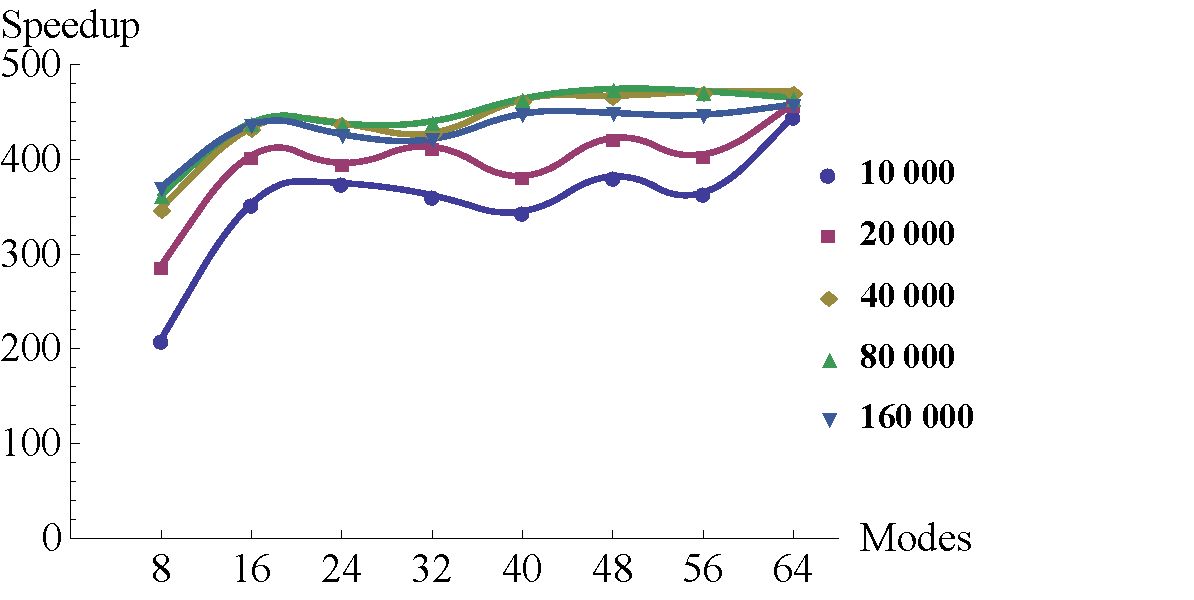
\includegraphics[width=\textwidth]{plot/SpaceChargeGPU11th_large.pdf}
        \caption{空间电荷效应求解器加速比}
        \label{fig:SCOpt}
    \end{subfigure}
    \quad
    ~ %add desired spacing between images, e. g. ~, \quad, \qquad, \hfill etc.
      %(or a blank line to force the subfigure onto a new line)
    \begin{subfigure}[b]{0.9\textwidth}
        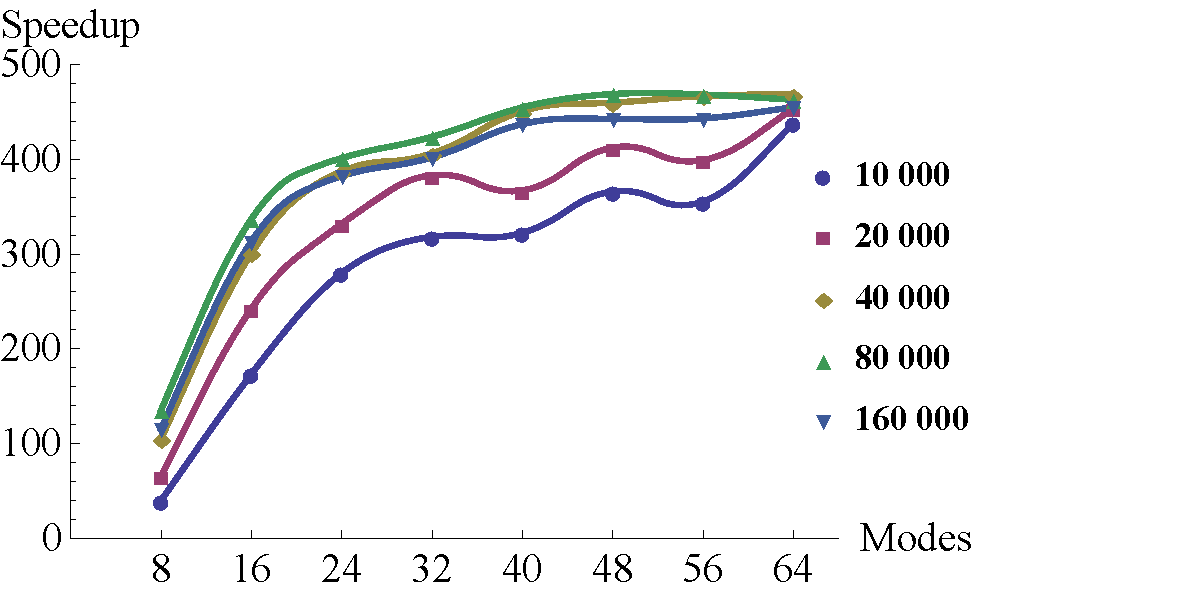
\includegraphics[width=\textwidth]{plot/TotalGPU11th_large.pdf}
        \caption{程序整体加速比}
        \label{fig:TotalOpt}
    \end{subfigure}
    \caption{单GPU加速比}\label{fig:OneGPU}
\end{figure}

图\ref{fig:SCOpt}为优化后的空间电荷效应求解器的加速比在不同的问题规模下的变化。其中,横坐标为展开的阶数,而纵坐标是加速比,不同的线是不同粒子数目的结果。可以看到,阶数越大加速比越高,这与我们的预期符合,因为阶数越大意味着空间电荷求解器占用的时间在总时间中的比例越大。其中,在$8*8*8$阶时加速比很低,因为在这种模式下的计算量很低。随着阶数的增加,计算量也随之增加,GPU的负载更为平衡,因此取得了更大的加速比。另一方面,粒子数目对于加速比的影响很小,在大阶数的情况下尤为如此。这是因为粒子数目本身远远超出了一个GPU的核心数目(在GTX 1060 上为1280个核心),即时在最低粒子数(10000个粒子)的情况,程序也能有效的使用所有的核心,而随着粒子数目的轻微提升是因为GPU能够在更大运算量的情况下更好的协调和平衡计算资源。

图\ref{fig:TotalOpt}为程序整体的运行时间的加速比,除了空间电荷效应求解之外,程序总体运行时间还包括外部传输矩阵,从Z坐标到T坐标的变换,粒子信息统计以及输入输出。
同空间电荷效应求解器相比,整体时间的加速比在各个问题规模下都略有下降,但是加速比变化的趋势却保持一致。
其中,在低阶情况下,比如$8\times8\times8$阶或$16\times16\times16$阶,因为空间电荷效应求解器所占总时间的比重不大,所以加速比的下降更为严重。
然而,在高阶情况下,空间电荷效应求解所占的时间会占总时间的绝大部分,所以总时间的加速比和空间电荷效应求解的加速比能够基本保持一致。

总之,我们取得了非常好的加速比。对于程序整体的总运行时间,优化的GPU代码比CPU代码运行速度高450倍;而如果仅仅比较空间电荷效应求解器,其最大加速比超过了460。

\subsection{多GPU性能提升-泰坦}
泰坦使用CPU和GPU混合架构,是目前世界上最快,规模最大的计算机集群之一。泰坦的每个节点拥有一个AMD Opteron(16核心)的CPU和一个NVIDIA Tesla K20x (2688核心)的GPU。为了测试多GPU的程序可扩展性,我们最多使用了1024个节点进行测试。其中,为了在不同节点的GPU上交换信息,我们需要先把GPU上的数据拷贝到CPU侧,再使用MPI协议在不用节点之间交换数据,最后再将交换后的信息拷贝回GPU侧。
在本次测试中,我们使用16$\times$16$\times$16阶进行测试,使用这个阶数是为了精确度和计算速度之间的平衡,也是我们在实际模拟中最常用的阶数。
如图\ref{fig:Titan}所示,我们分别讨论了空间电荷效应和整个程序在不同的粒子数目下,在不同的节点数上的加速比。其中,横轴为节点数目,纵周围加速比,加速比有多节点的运行时间除以单节点的运行时间得到,不同线是不同粒子数目的结果。

\begin{figure}[!htb]
    \centering
    \begin{subfigure}[b]{0.9\textwidth}
        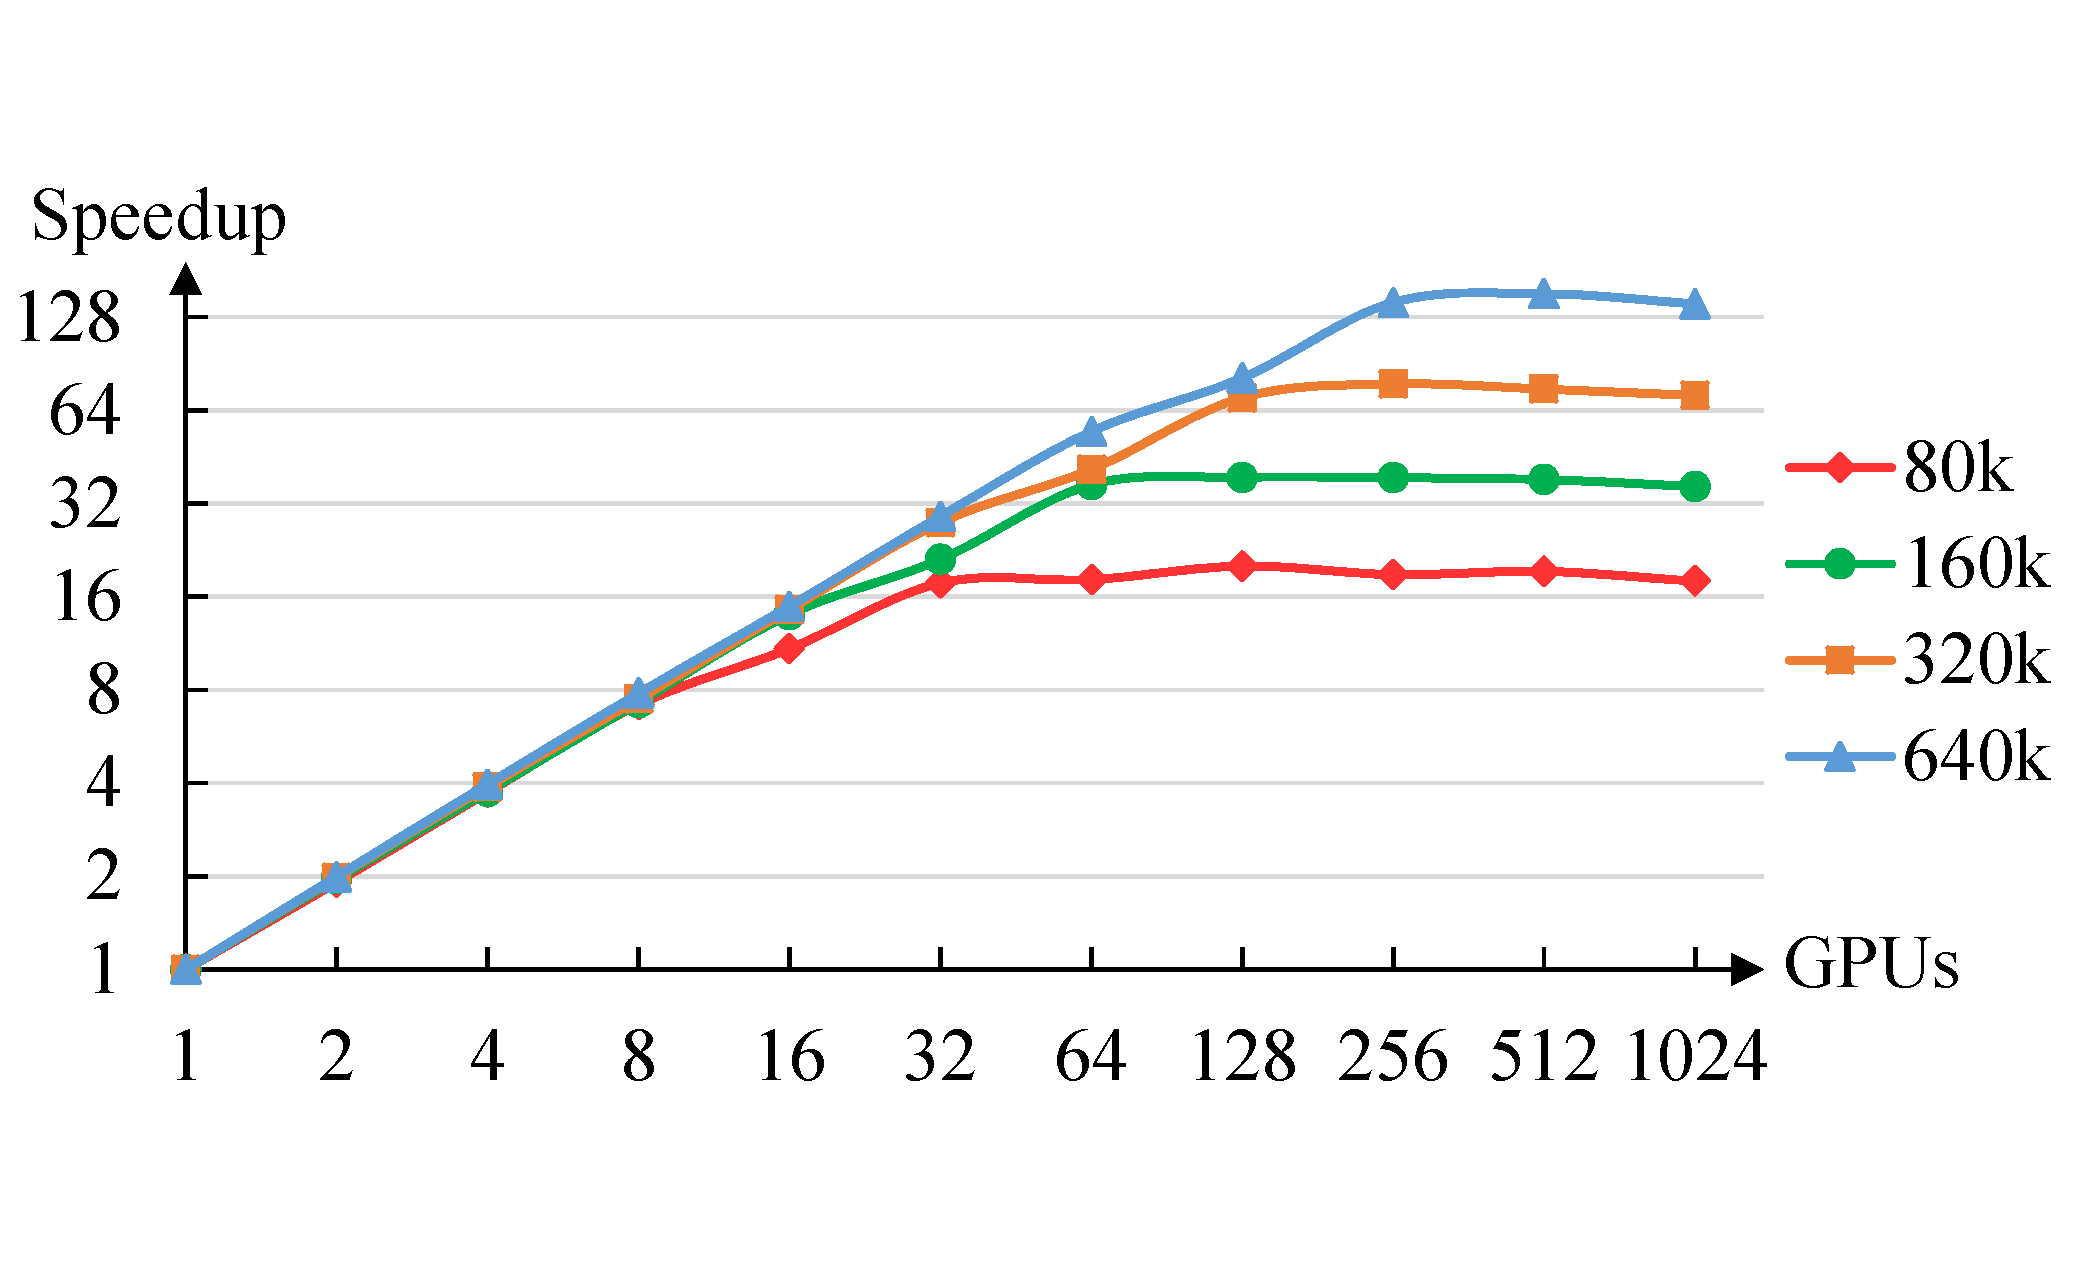
\includegraphics[width=\textwidth]{plot/640k_speedup_of_space_charge_kicker5log.pdf}
        \caption{空间电荷效应求解器加速比}
        \label{fig:SCTitan}
    \end{subfigure}
    \quad
    ~ %add desired spacing between images, e. g. ~, \quad, \qquad, \hfill etc.
      %(or a blank line to force the subfigure onto a new line)
    \begin{subfigure}[b]{0.9\textwidth}
        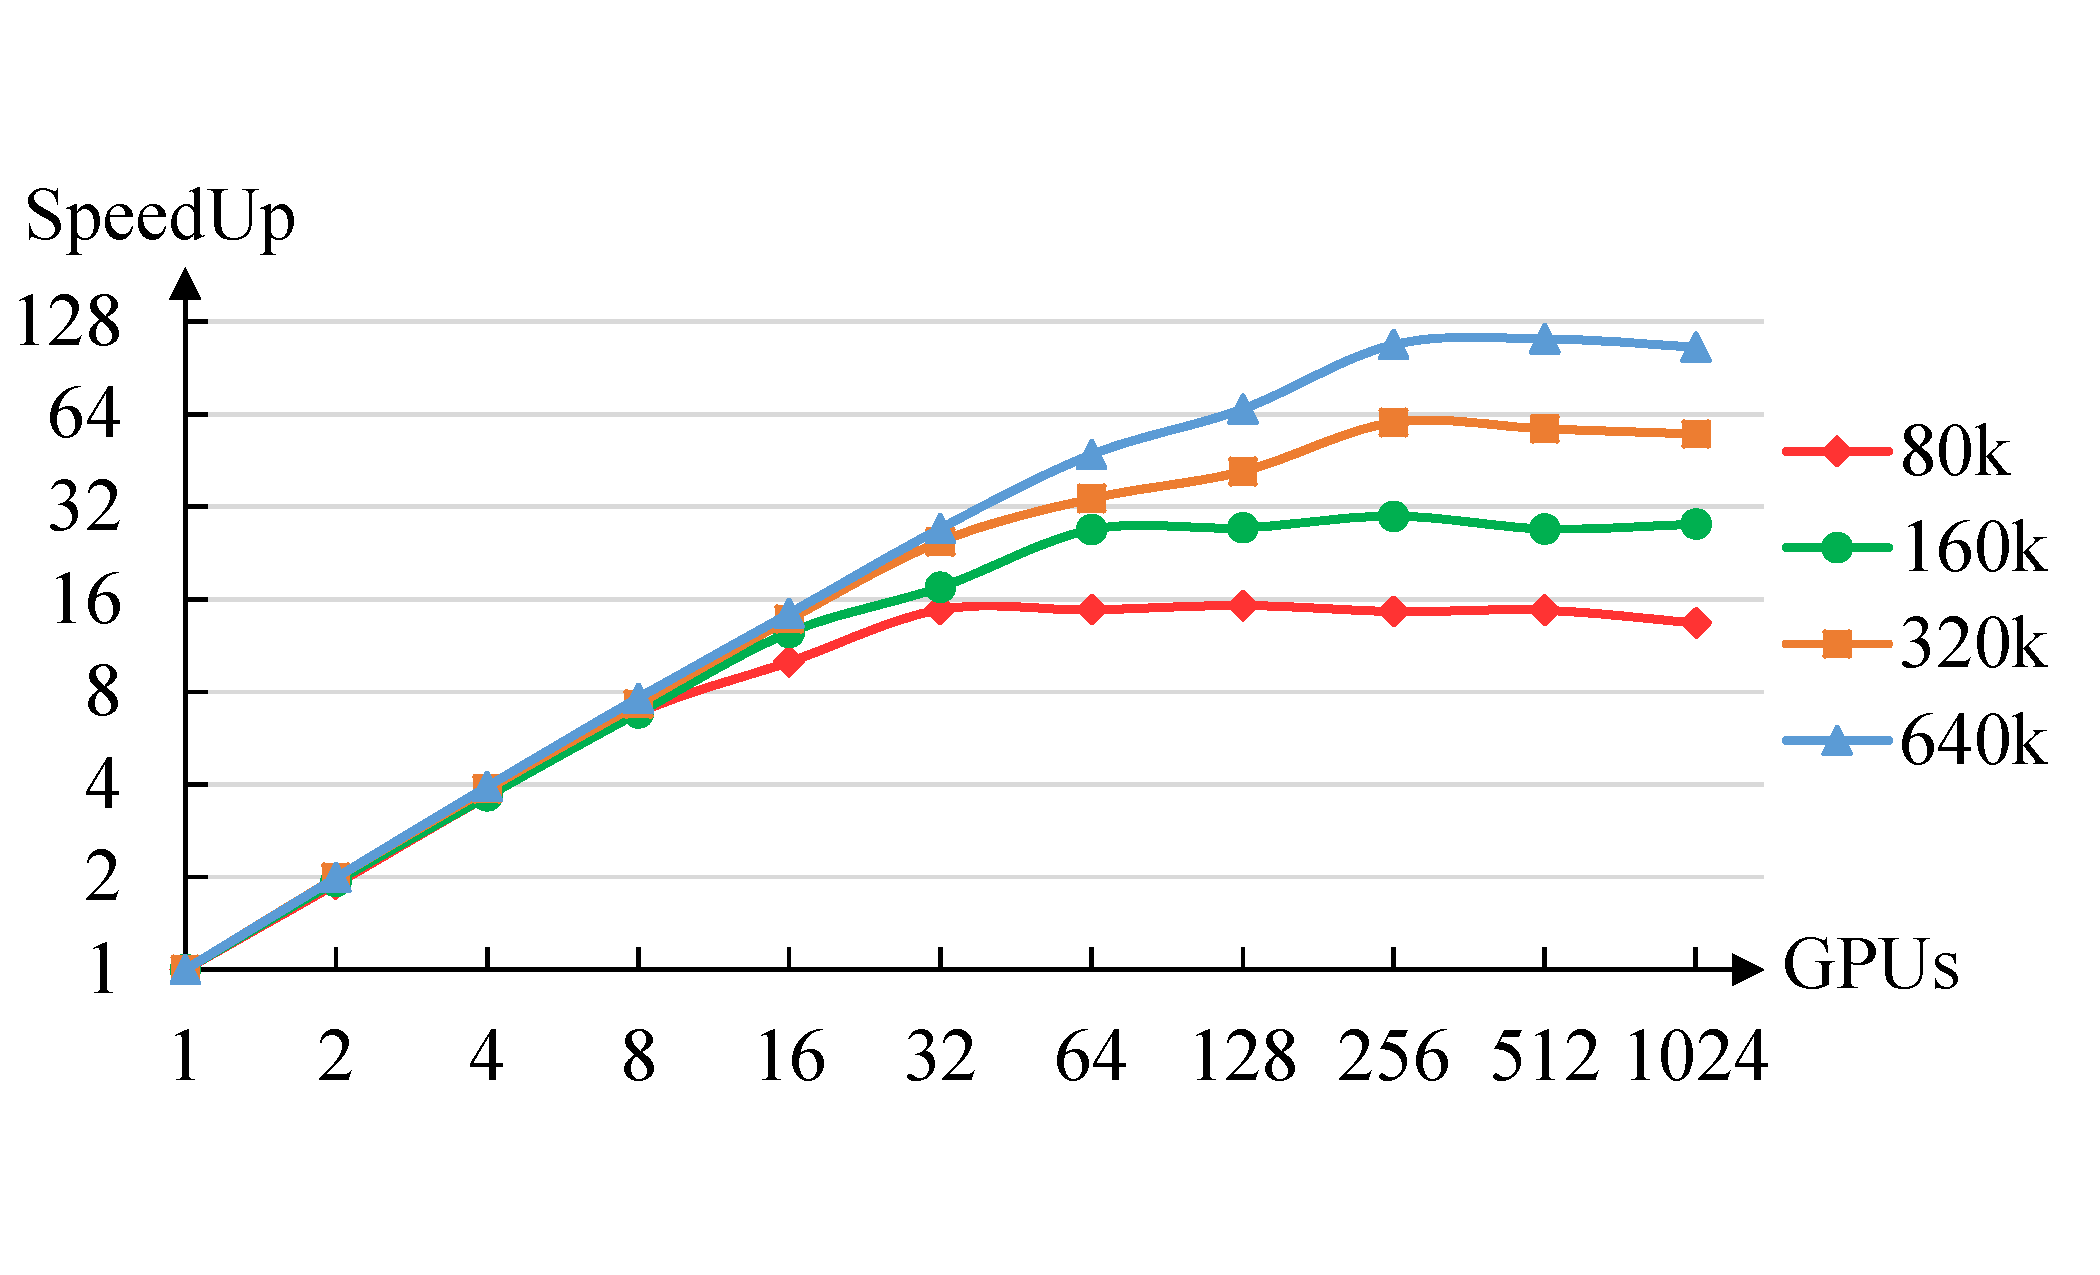
\includegraphics[width=\textwidth]{plot/640k_speedup_of_looptime5log.pdf}
        \caption{程序整体加速比}
        \label{fig:TotalTitan}
    \end{subfigure}
    \caption{多GPU加速比}\label{fig:Titan}
\end{figure}

由图\ref{fig:SCTitan}可得,在一开始,空间电荷效应求解器的加速比随着GPU的数目几乎线性增加,随后,加速比逐渐到达一个极限。
一方面,加速比的线性增长主要是因为GPU之间的数据交换量很少。这是无网格保辛粒子跟踪算法的一个很大的优势,其数据交换量仅与模式数量有关,而与粒子数量无关。
另一方面,它可以实现的最大加速度主要受粒子数量的限制,线性增加的范围和极限也随着粒子数量的增加而增加。以160000粒子为例,加速比最大可以达到40。在Titan集群上,每个GPU包含2688个内核,当使用64个GPU时,我们使用了64 $\times$ 2688 = 172032个内核,即使用的核心数多于粒子数。在这种情况下,我们无法通过简单地使用更多的GPU来获得进一步加速。而粒子数目增加时,比如320000个粒子或640000个粒子,所能够使用的GPU数目也会随之增加,最大加速比和线性范围也就会增加。

图\ref{fig:TotalTitan}是程序整体总时间的加速比,其中外部传输矩阵,坐标变换,粒子信息统计这些部分也是并行化的。但是因为它们的计算量较低,很难取得很高的并行度。所以加速比略微下降。
\section{模拟}                \label{section:simulation}
我们使用这套保辛算法在周期聚焦结构中进行粒子跟踪和模拟。我们使零流强的周期相移为86.3259度,如果将10个周期视为一个环,则环的工作点为2.3979。随着流强的增加,相移会被压缩,工作点会在0.6A左右穿过2.3333的三阶共振线。环中还存在一个六极磁铁。

图\ref{fig:emitGrowthCompare}为不同流强下的束流发射度增长变化,可以看到,发射度在流强为0.1A 和0.2A 时基本保持不变,这时的工作点约为2.40。但是发射度在流强为0.4A,0.6A,和0.8A时持续增长,这时的工作点在2.3333附近,可知其发射度增长是由于三阶共振导致。

\begin{figure}[!htb]
    \centering
    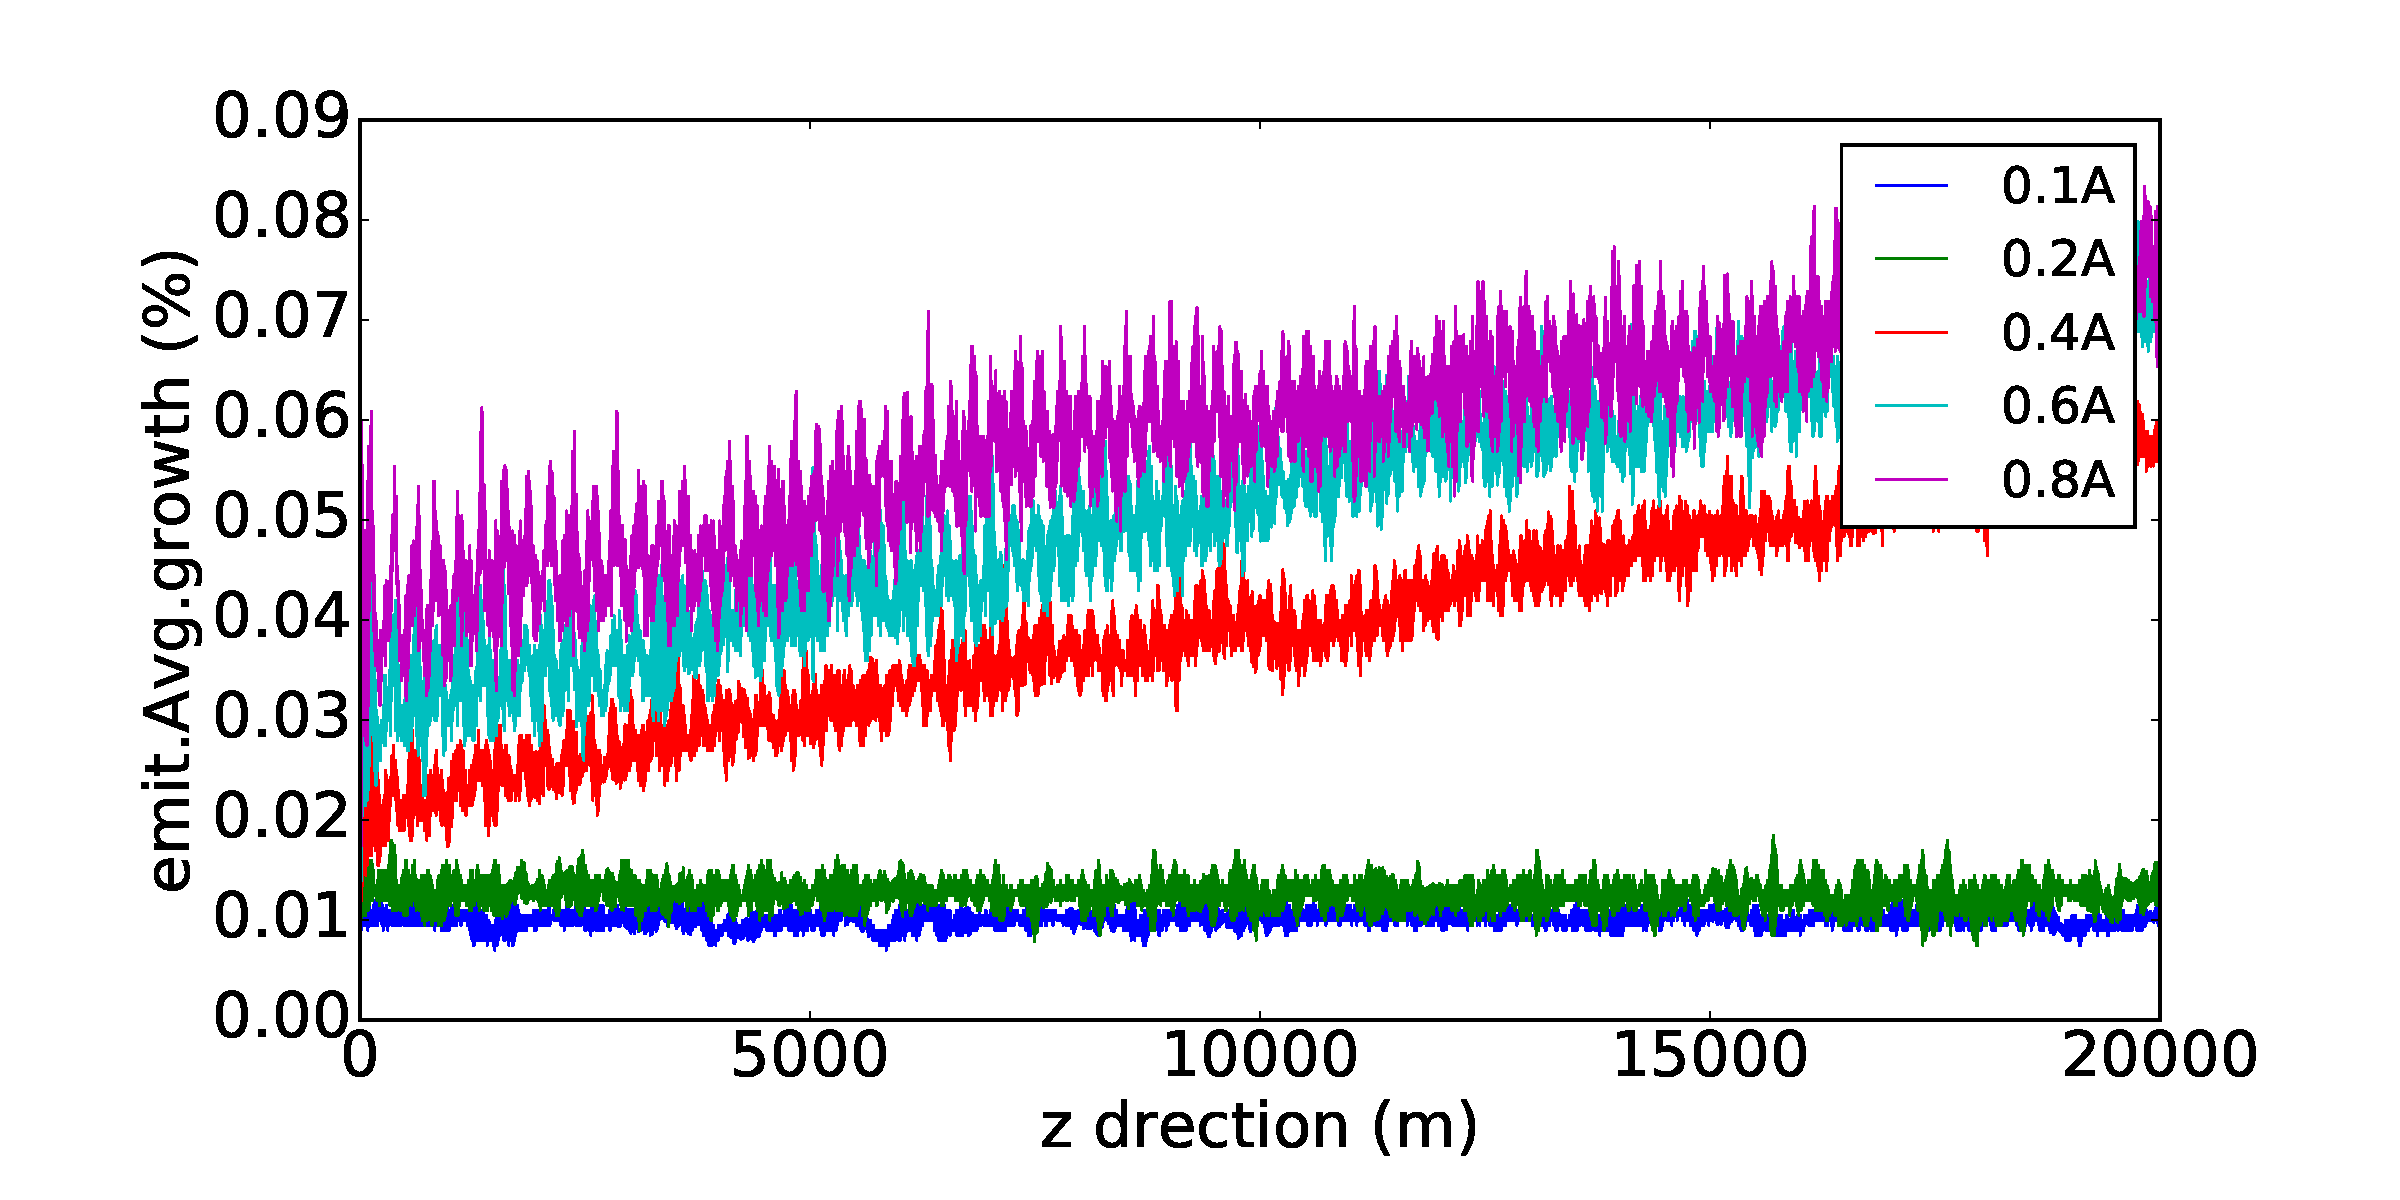
\includegraphics[width=\textwidth]{plot/emitGrowthCompare.pdf}
    \caption{不同流强下的发射度增长}
    \label{fig:emitGrowthCompare}
\end{figure}

图\ref{fig:Poincare}是工作点为2.3333附近时的粒子坐标的庞加莱截面,其中颜色越暗表示粒子密度越大,而不同的图片代表粒子处于不同的初始位置。受空间电荷效应驱动,庞加莱截面会被被扭曲,并塑造成三角形形状。受到三阶共振影响的粒子的横向位置会逐渐变大。最后,粒子会成为束晕的一部分并丢失。

\begin{figure}[!htb]
    \centering
    \begin{subfigure}[b]{0.48\textwidth}
        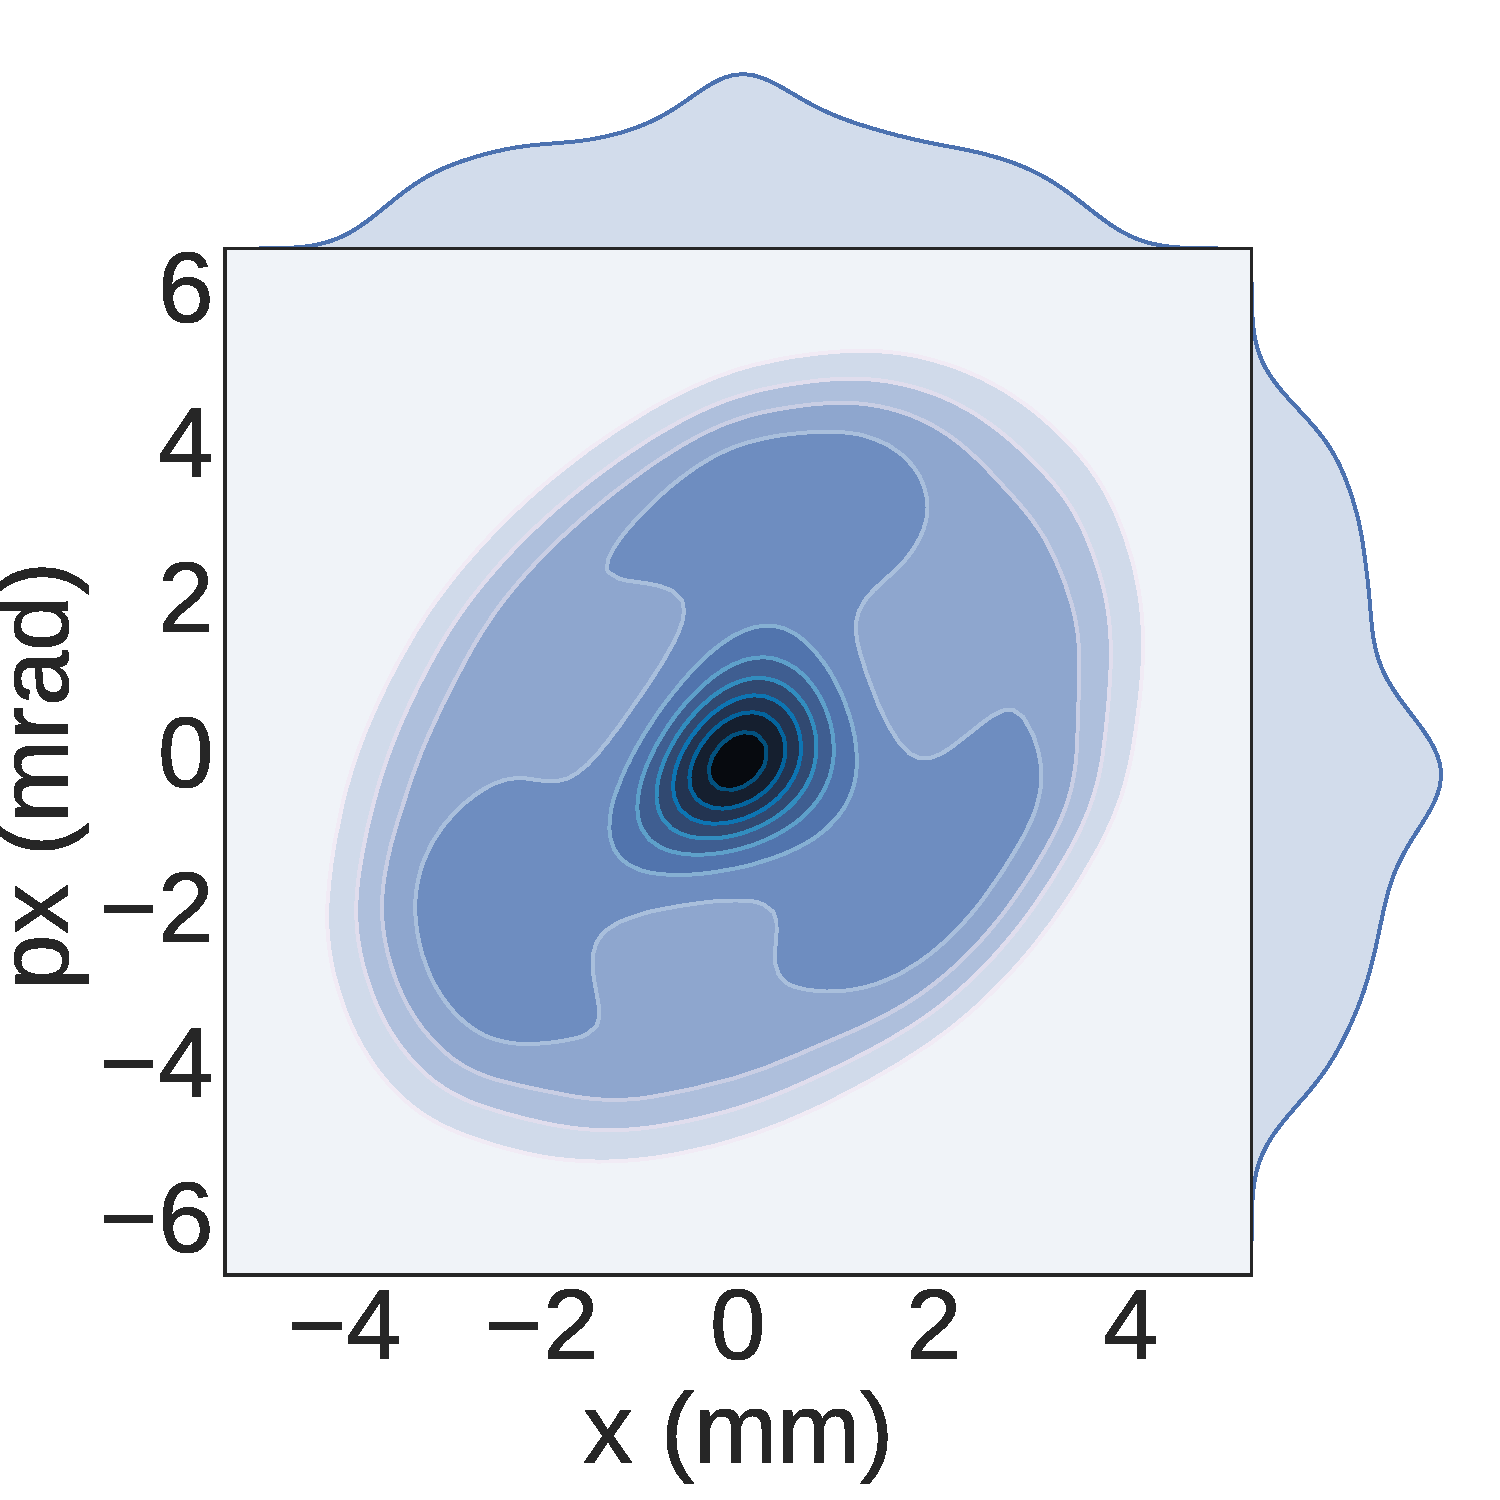
\includegraphics[width=\textwidth]{plot/particle_contour_nlevel9/sptc00002_xpx.pdf}
        \caption{}
    \end{subfigure}
    \begin{subfigure}[b]{0.48\textwidth}
        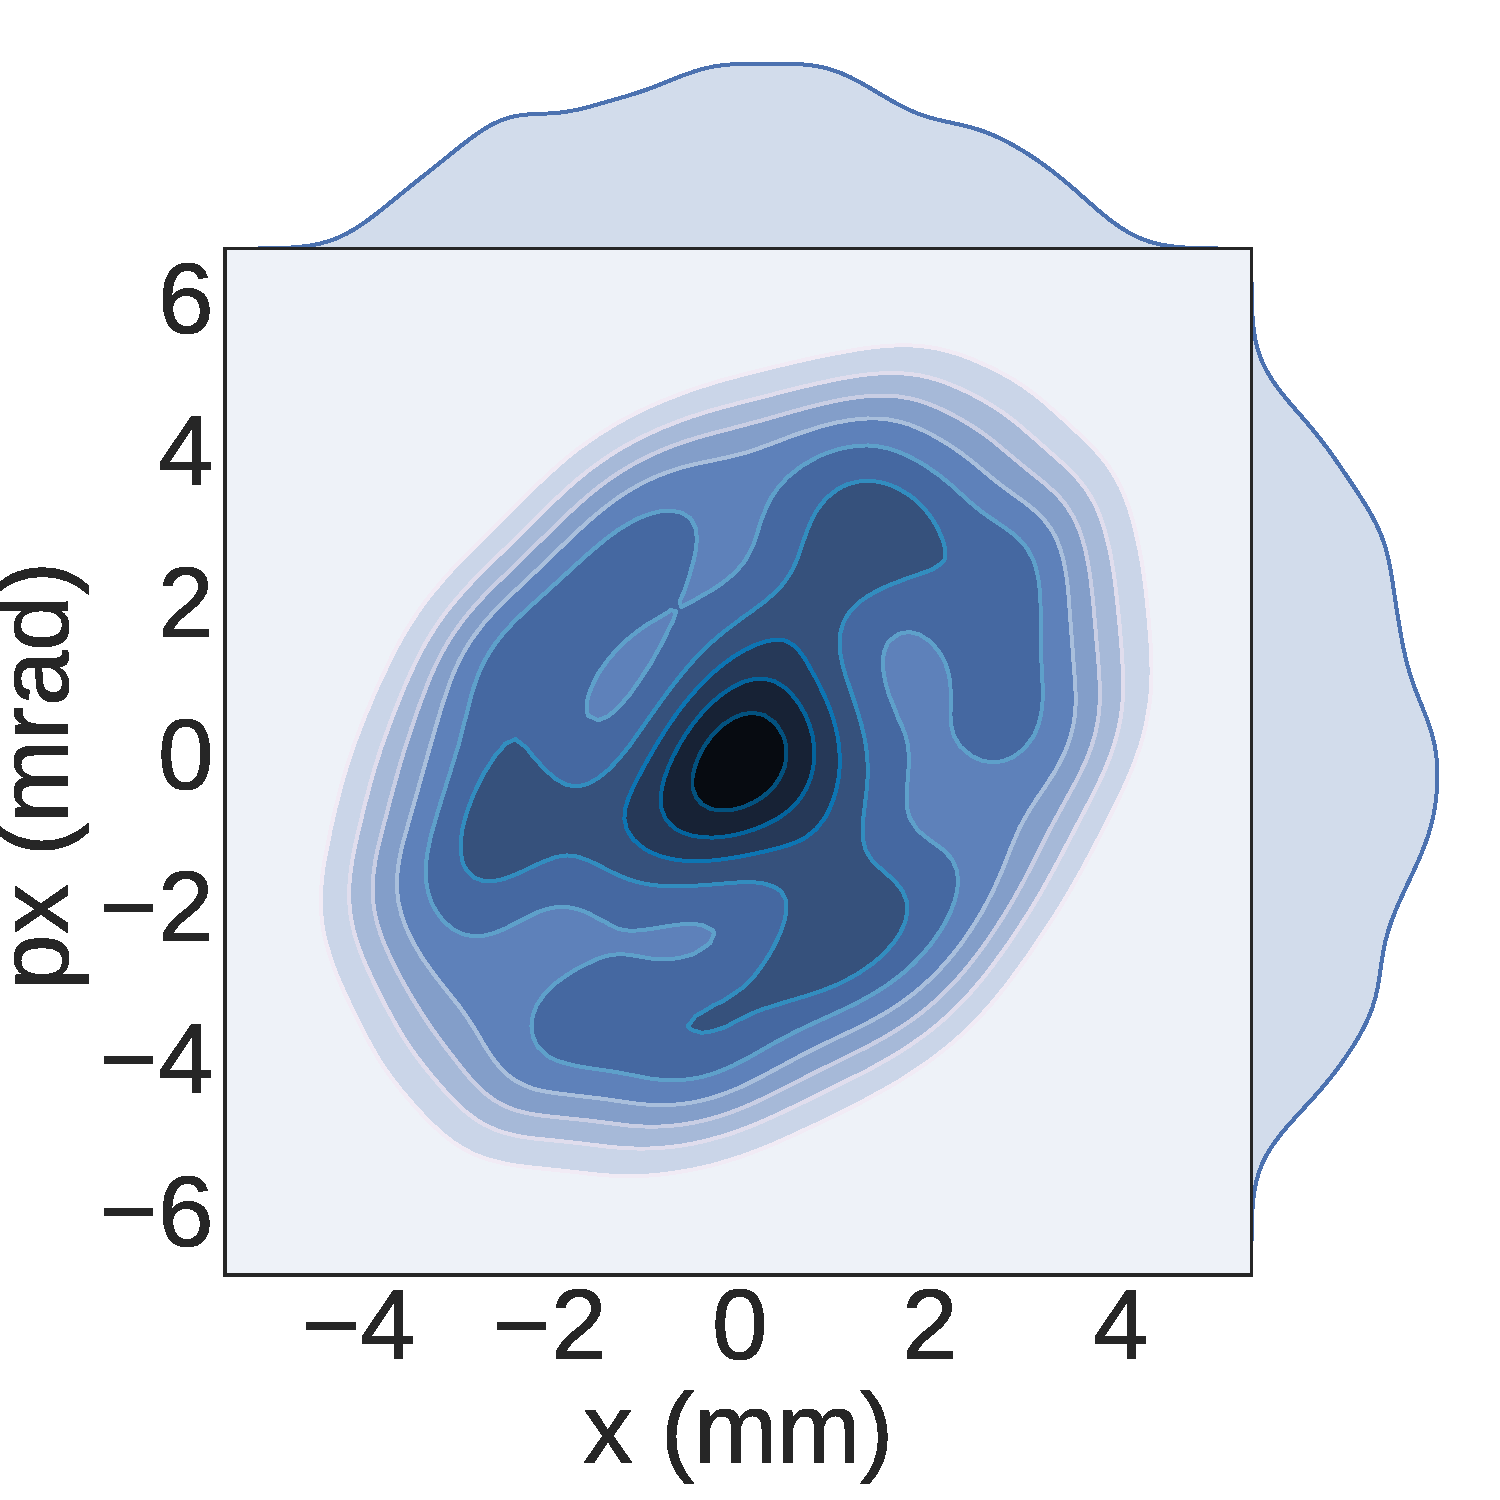
\includegraphics[width=\textwidth]{plot/particle_contour_nlevel9/sptc00005_xpx.pdf}
        \caption{}
    \end{subfigure}
    \begin{subfigure}[b]{0.48\textwidth}
        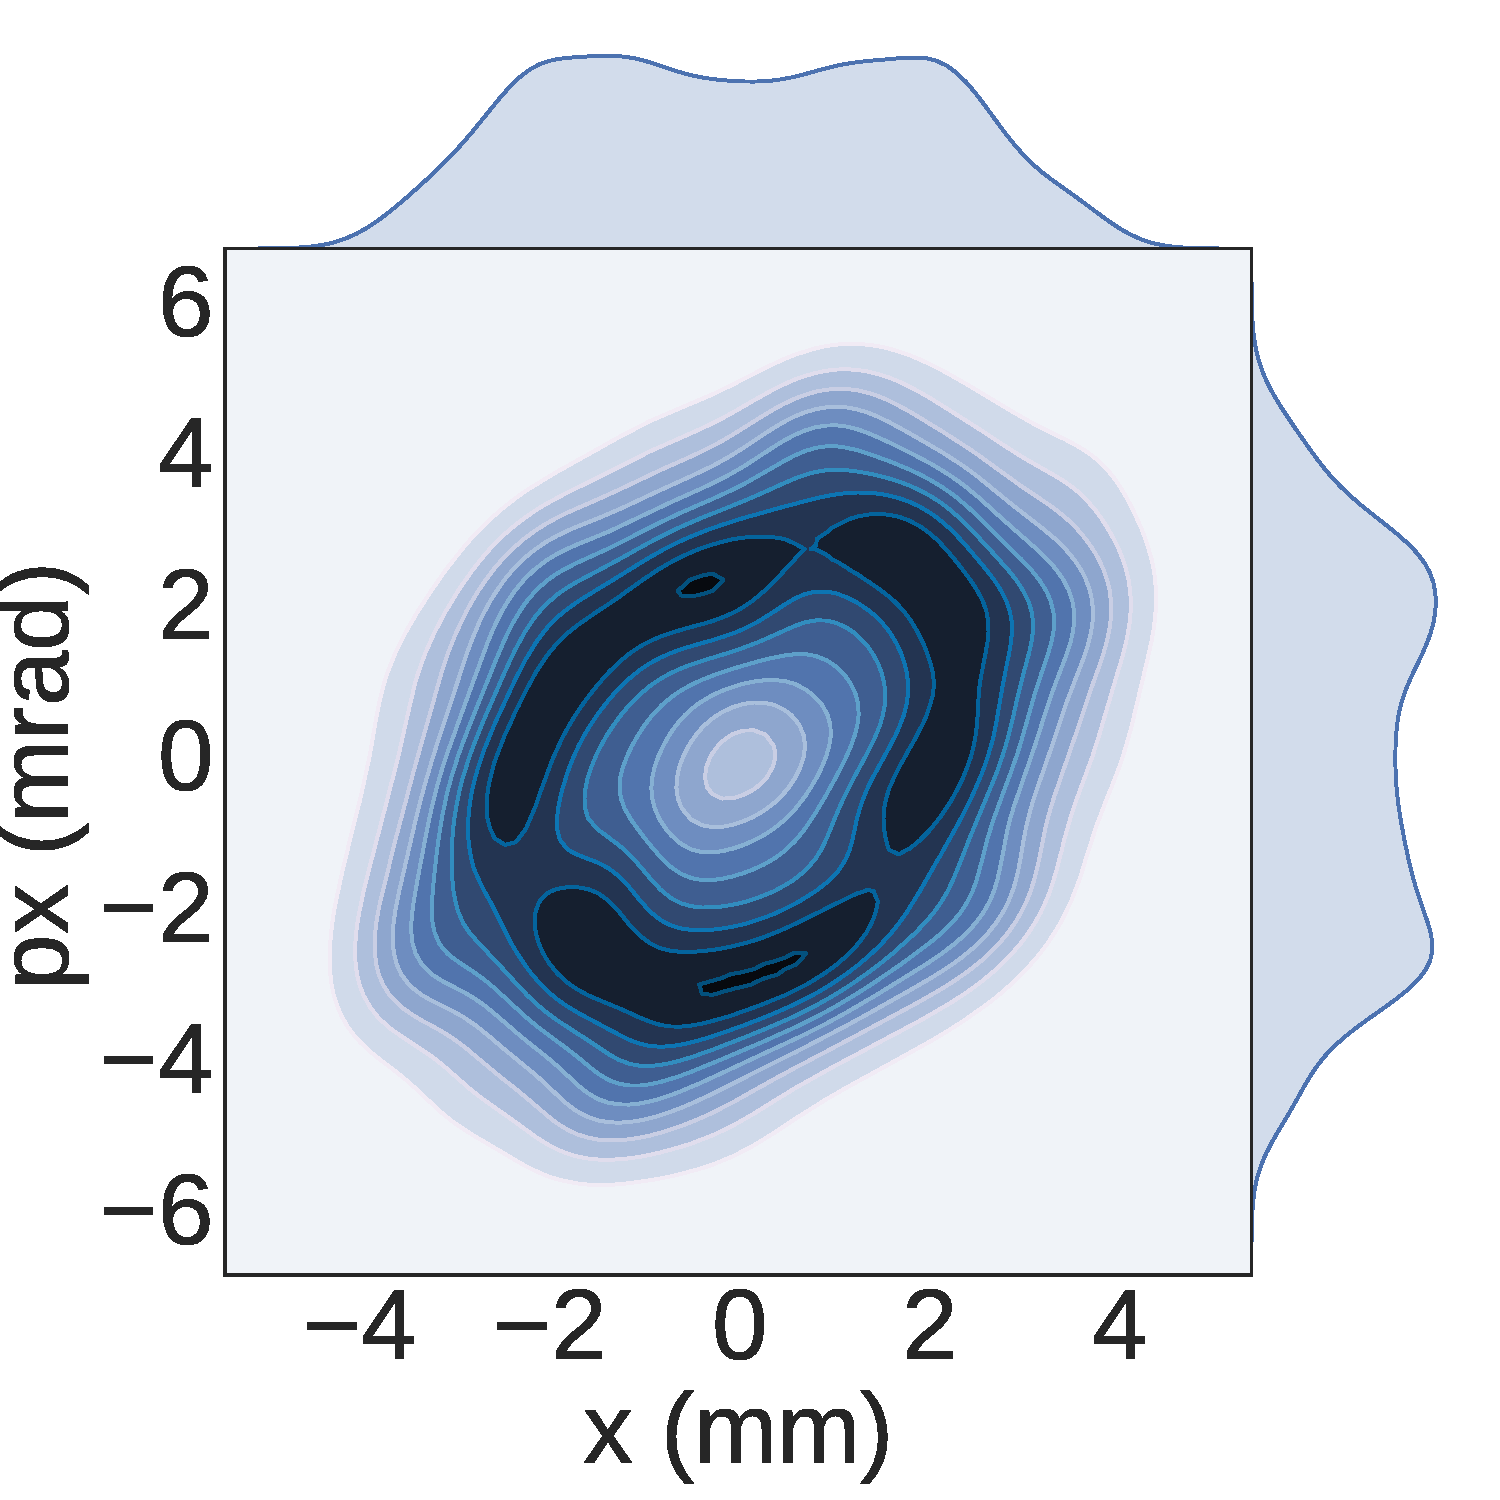
\includegraphics[width=\textwidth]{plot/particle_contour_nlevel9/sptc00003_xpx.pdf}
        \caption{}
    \end{subfigure}
    \begin{subfigure}[b]{0.48\textwidth}
        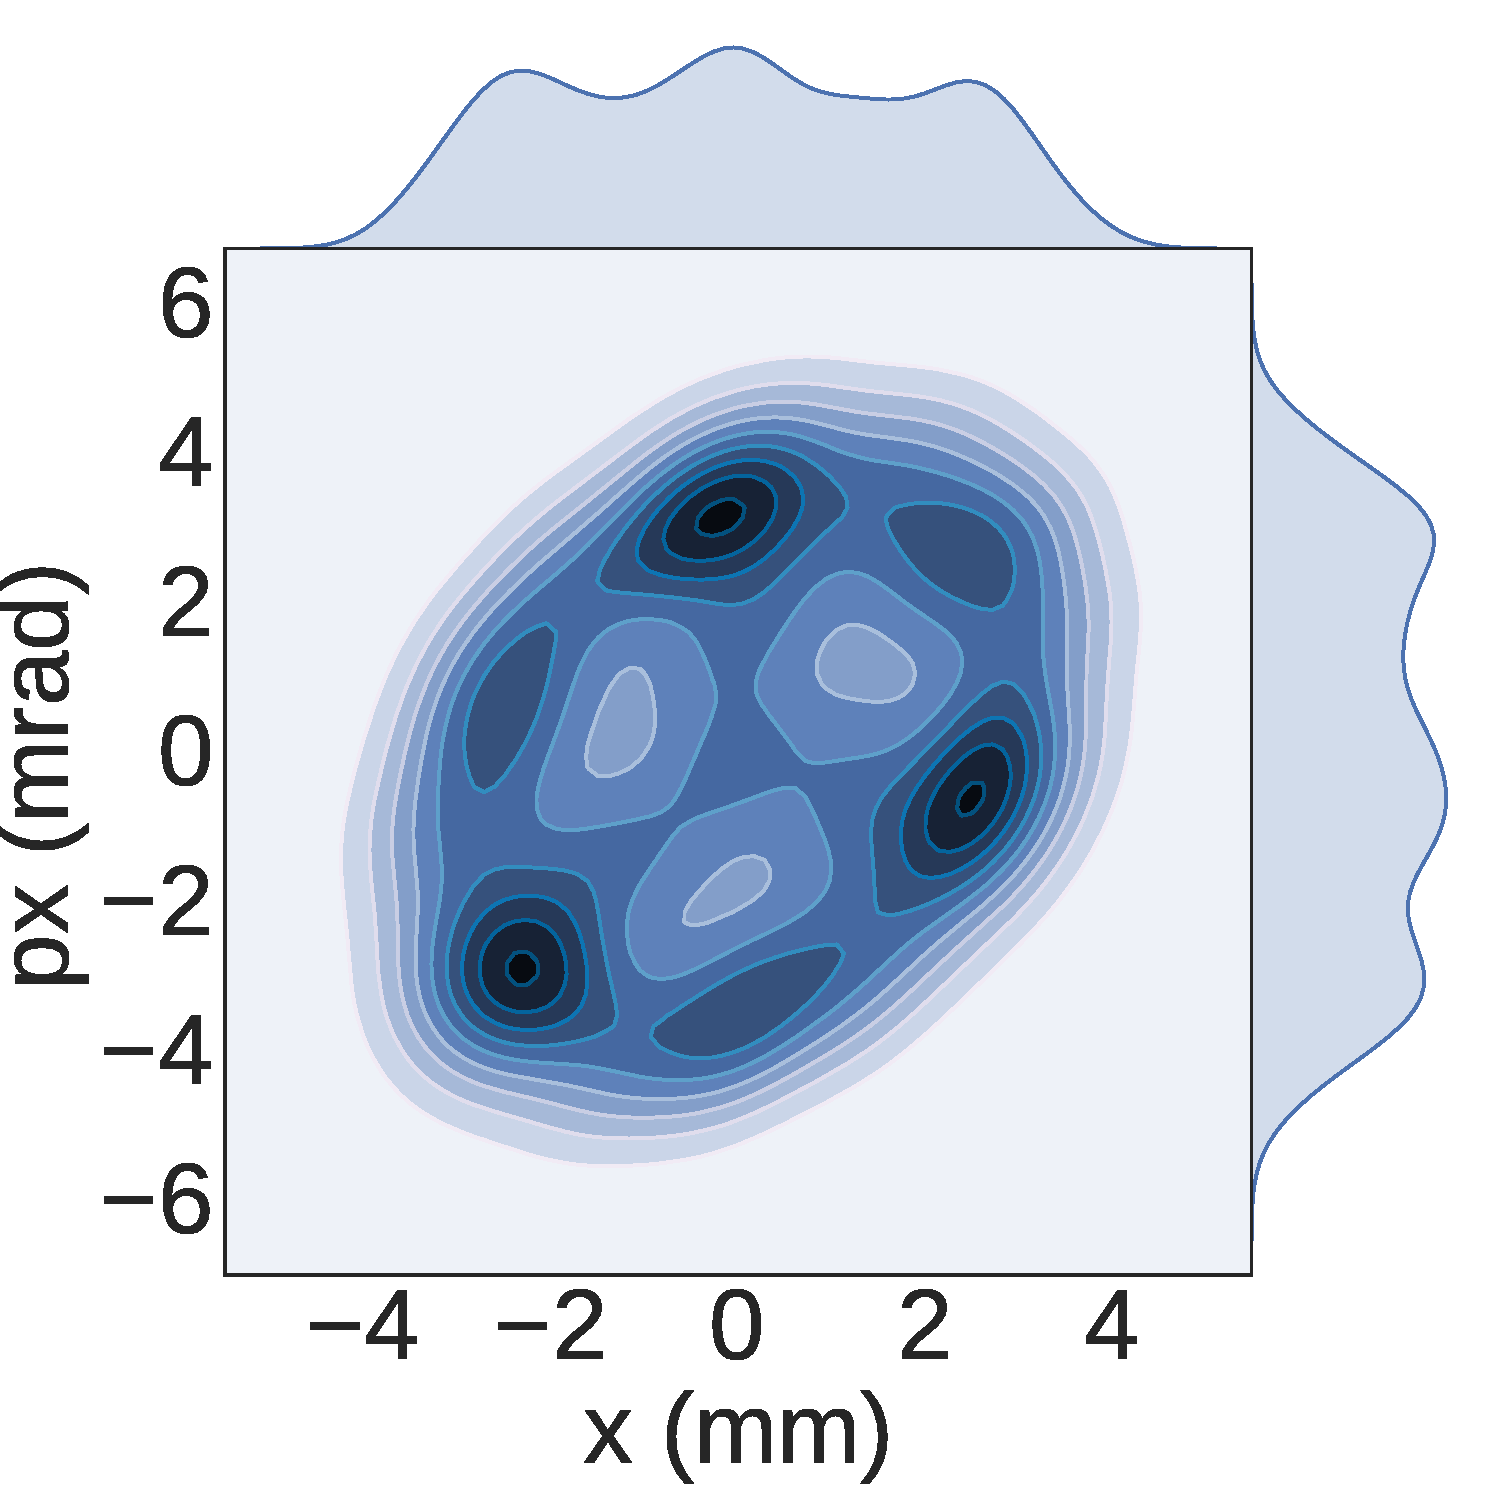
\includegraphics[width=\textwidth]{plot/particle_contour_nlevel9/sptc00006_xpx.pdf}
        \caption{}
    \end{subfigure}
    \caption{三阶共振附近的庞加莱截面}\label{fig:Poincare}
\end{figure}

\section{小结}                \label{section:conclusion}
我们使用CUDA库在GPU上实现了无网格保辛粒子跟踪算法。这个算法能够保障辛条件并有效降低由于网格热效应带来的发射度增长。
在一个普通家用GPU上,程序获得了超过450倍的加速比。同时,我们在GPU集群泰坦上的测试还显示出这种算法有良好的可扩展性,程序的加速比随着GPU数目几乎线性增加。
我们在周期性聚焦结构中使用这个程序进行了几个应用模拟,当工作点远离共振线时,束流不会出现发射度增长,而当其接近共振线时发射度会持续增长。
在未来的研究中,我们将继续扩展此程序,在不同架构的计算机上比较保辛算法的效率。